%
%  Thesis Vorlage für die Hochschule Heilbronn
%
%  Created by Prof. Dr. Detlef Stern on 2010-08-14.
%  Updated by Valentin Weber on 2020-10-05.
%  Copyright (c) 2020 . All rights reserved.
%
\documentclass[12pt,toc=bib,toc=listof]{scrreprt}
\usepackage[ngerman]{babel} 
\usepackage[utf8]{inputenc}
\usepackage[T1]{fontenc}
\usepackage{lmodern}
\usepackage{float}
\usepackage{setspace}
\usepackage{geometry}
\usepackage{amsthm}
\usepackage{amsmath}
\usepackage{amssymb}
\usepackage{graphicx}
\usepackage[style=apa,backend=biber]{biblatex}
\addbibresource{Quellen.bib}
\usepackage{hyperref}
\hypersetup{
  ,colorlinks=true
  ,linkcolor=black
  ,citecolor=black
  ,filecolor=black
  ,urlcolor=black
  }

% Fachbezogene Werte (müssen aktualisiert werden)
\newcommand{\hhnthesis}{Bachelor Thesis}
\newcommand{\hhnthesisnum}{173312}
\newcommand{\hhnsubject}{Angewandte Informatik}
\newcommand{\hhnsubjectnum}{SPO1a}
\newcommand{\hhnlecturer}{Prof. Dr. rer. nat. Nicole Ondrusch}

% Vom Studierenden zu aendernde Werte
\newcommand{\reprttopic}{Einsatz von Künstlicher Intelligenz zur Testfallgenerierung}
\newcommand{\reprtstudentname}{Marvin Müller}
\newcommand{\reprtstudentid}{212117}
\urldef{\reprtstudentmail}\url{mmueller3@stud.hs-heilbronn.de}

\usepackage[headsepline]{scrlayer-scrpage}
\pagestyle{scrheadings}
\clearscrheadfoot
\ihead{\reprttopic}
\ohead{\pagemark}
\renewcommand*{\chapterpagestyle}{scrheadings}
\renewcommand*{\chapterheadstartvskip}{}

% Deckblatt Definitionen (begin)
\titlehead{\flushright
\includegraphics{./Bilder/hhn.png}}
\subject{{\hhnthesis{} (\hhnthesisnum{})}\\{\hhnsubject{} (\hhnsubjectnum{})}}
\title{\reprttopic}
\author{\reprtstudentname\footnote{\reprtstudentid, \reprtstudentmail}}
%% Datum nie auf einen festen Wert setzen
\publishers{Eingereicht bei \hhnlecturer}
% Deckblatt Definitionen (end)

\begin{document}
\pagenumbering{Roman} 
\selectlanguage{ngerman}
\maketitle
\newgeometry{left=25mm, top=25mm, right=25mm, bottom=25mm}

\tableofcontents

\addchap{Abkürzungsverzeichnis} % (fold)
\label{sec:abkuerzungsverzeichnis}

\begin{description}
  \item[AI:] Artificial Intelligence
  \item[GUI:] Graphical User Interface (Deutsch: Grafische Benutzeroberfläche)
  \item[KI:] Künstliche Intelligenz
  \item[LLM:] Large Language Model (Deutsch: Großes Sprachmodell)
  \item[NLP:] Natural Language Processing (Deutsch: Verarbeitung natürlicher Sprache)
  \item[RAG:] Retrieval Augmented Generation
\end{description}

\newpage
\listoffigures
\newpage
\addchap{Gender Hinweis} % (fold)
\label{sec:genderHinweis}
In dieser Bachelorarbeit aus Gründen der besseren Lesbarkeit das generische Maskulinum verwendet. Dabei gilt die männliche Sprachform für alle Geschlechter.
% chapter genderHinweis (end)

\addchap{Abstract} % (fold)
\label{sec:abstract}
This bachelor thesis investigates the use of artificial intelligence in the creation of requirement test cases, taking into account the requirement specifications provided by artificial intelligence. The aim of the work and the evaluation of the results was to find out whether artificial intelligence is able to generate requirement test cases that achieve a higher test quality and test coverage than requirement test cases created by humans/developers. The same requirement specifications were used and the test cases were compared with each other. The intention was to contribute to the improvement of test case generation.\\
The results of this bachelor thesis show that
\\
\textbf{Keywords:} AI, LLM, RAG, Prompting, Test Case Generation
% chapter abstract (end)
\newpage

\addchap{Zusammenfassung} % (fold)
\label{sec:zusammenfassung}
Diese hier vorliegende Bachelorarbeit erforscht den Einsatz von Künstlicher Intelligenz bei der Erstellung von Anforderungstestfällen unter Berücksichtigung der Künstlichen Intelligenz zur Verfügung gestellten Anforderungsspezifikationen. Ziel der Arbeit und der Auswertung der Ergebnisse war es herauszufinden, ob Künstliche Intelligenz dazu in der Lage ist, Anforderungstestfälle zu erzeugen, die eine höhere Testqualität und Testabdeckung erreichen als von Menschen/Entwicklern erstelle Anforderungstestfälle. Dabei wurden die gleichen Anforderungsspezifikationen verwendet und die Testfälle miteinander verglichen. Intention war es, einen Beitrag zur Verbesserung der Testfallgenerierung zu leisten.\\
Die Ergebnisse dieser Bachelorarbeit zeigen, dass
\\
\textbf{Stichwörter:} KI, LLM, RAG, Prompting, Testfallgenerierung
% chapter abkuerzungsverzeichnis (end)

\newpage
\pagenumbering{arabic}

% report (begin)
\chapter{Einleitung} % (fold)
\label{sec:einleitung}
Über die Motivation und das Ziel der Bachelorarbeit wird in Kapitel 1 Einleitung eingegangen.

\section{Motivation} % (fold)
\label{sec:motivation}
In den vergangenen Jahren hat in dem Bereich Künstliche Intelligenz (KI) eine rasante Entwicklung stattgefunden. Diese hat dabei eine Auswirkung auf das private als auch auf das geschäftliche Leben. Der Artikel des Branchenverbandes der deutschen Informations- und Telekommunikationsbranche - Bitkom - führt die von ihnen durchgeführte Studie auf (\cite{StreimHecker2023}). Nach dieser hat sich der Anteil der deutschen Unternehmen, welche KI nutzen, von 9\% im Jahr 2022 auf 15\% im Jahr 2023 nahezu verdoppelt. Dabei sehen 68\% der Befragten KI als Chance.\\
\\
In einer Pressemitteilung vom 25. November 2024 gibt das Statistische Bundesamt bekannt, dass bereits 20\% der in Deutschland ansässigen Unternehmen KI verwenden (\cite{StatistischesBundesamt2024}). Dabei sind die drei häufigsten Einsatzbereiche für KI Textmining - Analyse geschriebener Sprache mit 48\%, Spracherkennung mit 47\% und die Erzeugung von natürlicher Sprache mit 34\%. Dies zeigt eine rasante Steigerung der Nutzung von KI alleine in den letzten drei Jahren und es lässt sich erkennen, dass KI bereits vielfältig einsetzbar und nutzbar ist. Gerade in der Informatik und der Softwareentwicklung.\\
\\
In dieser Arbeit stehen KI Sprachmodelle im Vordergrund. Diese sogenannten Large Language Models (LLM) bieten sich  dafür an, redundante und sich ähnliche Aufgaben für den Anwender zu erledigen (\cite{Kerner2024}). Gut geeignet ist dafür die Textgenerierung durch LLM. LLM werden deshalb bereits in verschiedensten Bereichen der Textgenerierung verwendet. Zu nennen sind dabei Übersetzung, Texterstellung, Textzusammenfassung, Kategorisierung und Klassifizierung. Eine Anwendungsmöglichkeit der Textgenerierung ist deshalb die Testfallgenerierung durch die KI. Das Erstellen von Testfällen mithilfe von KI kann erhebliche Zeit- und Kosteneinsparungen für Unternehmen und Tester ermöglichen.\\
\\
Ein Testfall hat eine Struktur, welche definierten Regeln entspricht. In der Softwareentwicklung, aber auch allgemein in fast allen beruflichen und wissenschaftlichen Bereichen wird getestet. Somit ist die Testfallgenerierung durch KI nahezu universell einsetzbar. Es gibt bereits KI Tools und Arbeiten, welche sich mit dem Thema KI erzeugte Testfälle beschäftigt haben. Zu nennen sind dabei die Werke von (\cite{Bozic2022}) und (\cite{WeingartzSuleymanov2024}). Vorteile von KI generierten Testfälle sind dabei eine gesteigerte Qualität und Kosten und Zeiteinsparungen.\\
\\
In einer Arbeit wird die Wirksamkeit von LLM bei der Erstellung von Unit Tests untersucht (\cite{Ouédraogo2024}). Dabei kommen die Autoren zu dem Schluss, dass die mit LLM erzeugten Junit Tests den von Menschen geschriebenen Tests in Bezug auf Codierungsstandards sehr ähneln.\\
\\
Um das Thema des des automatischen GUI Testings beschäftigt sich eine weitere Arbeit (\cite{Liu2024}).
Dabei sehen sie einen großen Fortschritt im Bereich des automatischen GUI Testing, kommen jedoch zu der Erkenntnis, dass von LLM erzeugte Tests noch eine geringe Aktivitätsabdeckung aufweisen.\\
\\
Wie bei allen neuen Technologien ist es essenziell, sich auch der damit verbundenen Risiken bewusst zu sein. Ein Nachteil der KI ist zum Beispiel das Phänomen der Halluzination. Dieser Begriff beschreibt das Phänomen, dass eine KI Antwort, nicht mit den gegebenen Input übereinstimmt und faktisch nicht richtig ist (\cite{Siebert2024}).\\
\\
Ebenfalls ist der Umgang mit Daten nicht sicher. Ein mögliches Problem sind unternehmensinterne und auch persönliche Daten. Es gibt keine Transparenz darüber, wie diese behandelt werden, wenn sie einem LLM zur Verfügung gestellt werden(\cite{Möllers2024}). Persönliche Daten könnten missbraucht werden und LLM könnten mit unternehmensinternen Daten antrainiert werden, welche die Konkurrenz dann nutzen könnte. Daher stellt sich die Frage, ob es sinnvoller ist, ein eigenes Modell anzutrainieren, um die Sicherheit und Kontrolle über die Daten zu gewährleisten. Eine empfohlene Maßnahme für dieses Risiko ist die Anonymisierung persönlicher und sensibler Daten, bevor man diese der LLM zur Verfügung stellt.\\
\\
Da die im letzten Absatz beschriebene Lösung mit Zeit und Aufwand verbunden ist, bieten sich andere Methoden an und Modelle, welche Retrieval Augmented Generation (RAG) verwenden können, können sich gut für die Aufgabe der Testfallgenerierung eignen. Die Technik RAG beschreibt den Vorgang, dass das Wissen, welches das LLM benötigt, nicht aus dem Prompt - der Eingabe - kommen muss (\cite{Honroth2024}). Informationen aus Dateien, die dem LLM zur Verfügung gestellt werden, können ebenfalls verwendet werden.
% section motivation (end)

\section{Forschungsfrage} % (fold)
\label{sec:forschungsfrage}
Folgende Forschungsfrage soll untersucht werden und dient als Grundlage zur Durchführung der Arbeit. Sie ist dabei aus der Motivation entstanden.\\
\\
1. Ist es möglich, dass Large Language Models dazu in der Lage sind, aus Anforderungsspezifikationen Anforderungstestfälle zu erzeugen, welche eine höhere Testqualität und Testabdeckung aufweisen, als manuell erstellte Testfälle, die aus den gleichen Anforderungsspezifikationen erstellt werden?\\
% section forschungsfrage (end)
\newpage

\noindent
\section{Ziel der Arbeit} % (fold)
\label{sec:zielDerArbeit}
Ziel der Arbeit ist es, die Grundlagen und Anwendungsmöglichkeiten und -verfahren zu erforschen, durchzuführen und zu evaluieren.\\
Diese Bachelorarbeit soll ein Konzept und eine Vorgehensweise entwickeln, die sich für den Einsatz von KI für die Generierung von Anforderungstestfällen aus der KI zur Verfügung gestellten Anforderungsspezifikationen eignet. Diese stützt sich dabei auf bereits bestehender Vorgehensweisen und Modelle. Durch die theoretische und praktische Aufarbeitung, Erprobung und Verbesserung bestehender Vorgehensweisen und Modellen soll sie dabei ein Beitrag sein, die Effizienz und Qualität der mit Hilfe von KI erstellten Testfälle zu verbessern.
% section zielDerArbeit (end)

\section{Vorgehensweise} % (fold)
\label{sec:vorgehensweise}
Der Plan der vorliegenden Arbeit gestaltet sich wie folgt: Zuerst wird eine Literatur-
recherche durchgeführt. Dabei liegt der Fokus auf das Finden von bereits vorhandener
Vorgehensweisen und Modellen im Bezug auf Textgenerierung im Allgemeinen und Test-
fallgenerierung im Besonderen. Es ist ebenfalls notwendig, sich über Begriffe und Tech-
niken, welche während der Umsetzung der Arbeit notwendig sind, tiefer zu ergründen. 
Wichtig ist dabei zu ergründen, wie ein Testfall und eine Anforderungsspezifikation aufgebaut sind, welche Merkmale und welche Kriterien sie erfüllen müssen. Es muss erforscht werden, was eine KI ist, wie Modelle - LLM - aufgebaut sind und welche sich zur Testfallgenerierung eignen. Das Ermitteln geeigneter Prompting Methoden wie der Methode RAG ist ebenfalls erforderlich. Das Ziel ist dabei, die Untersuchung und Entdeckung bereits vorhandener Anwendungsmöglichkeiten, Vorgehensweisen und Modellen zur KI gesteuerten Testfallgenerierung.\\
\\
Nachdem passende Modelle und Vorgehen ermittelt wurden und passende Testdaten, welche sich in Anforderungsspezifikationen und aus diesen manuell erstellte Anforderungstestfälle gliedern, beginnt die praktische Umsetzung der Arbeit. Dabei liegt die Durchführung und Dokumentation der von der KI erstellten Anforderungstestfälle im Vordergrund.\\
\\
Zum Schluss werden die von der KI erstellten Anforderungstestfälle mit manuell erstellten Anforderungstestfälle verglichen und auf ihr Abschneiden im Bezug auf Testqualität und Testabdeckung ermittelt. Die Ergebnisse werden analysiert und hinsichtlich Aufwand, Durchführbarkeit und Richtigkeit ausgewertet. Dabei wird für die Auswertung Metriken verwendet, die in Kapitel 4 Methodik näher erläutert werden. Nachdem die Ergebnisse ausgewertet werden, gibt es eine Einordnung der Ergebnisse und eine Diskussion über mögliche zukünftige Entwicklungen in dem Bereich KI generierte Testfallerstellung.
% section vorgehensweise (end)
% chapter einleitung (end)

\chapter{Grundlagen und Hintergrund} % (fold)
\label{sec:grundlagenUndHintergrund}
Das Kapitel 2 Grundlagen und Hintergrund widmet sich den wissenschaftlichen Grundlagen und klärt über Begriffe und Methoden auf, die für das Verstehen und das Durchführen der Arbeit essenziell sind.

\section{KI} % (fold)
\label{sec:KI}
Diese Arbeit behandelt das Thema KI, deshalb ist es essentiell hier einen allgemeinen Überblick über dieses Thema zu geben.

\subsection{Allgemein} % fold
\label{sec:allgemein}
Der Begriff KI beziehungsweise im Englischen AI beschreibt ein Teilgebiet der Informatik. Dabei gibt es zwei Arten von KI. Erstens die schwache KI, welche auch als enge KI bezeichnet wird. Diese Art der KI kann nur einzelne und beschränkte Aufgaben lösen. Der Begriff KI wurde bereits im Jahr 1956 als Konzept vorgeschlagen. Seitdem entwickelte sie sich immer weiter. Im Jahr 1997 verliert der damalige Schachweltmeister Garry Kasparov gegen den Schachcomputer Deep Blue von IBM und im Jahr 2016 besiegt der Computer AlphaGo von Google Lee Se-dol, ein Go-Meister aus Südkorea. Diese Erfolge zeigen die Entwicklung der KI, sind jedoch auf die schwache KI beschränkt (\cite{Bhatt2021}), (\cite{Hecker2018}), (\cite{Mocko2021}), (\cite{Roscher2025}) und (\cite{Zhu2021}).Als Zweites gibt es das Konzept der starken KI, auch als allgemeine KI bekannt. Folgende Grafik zeigt, wie diese ihre Umgebung wahrnimmt.
\begin{figure} [H]
    \centering
    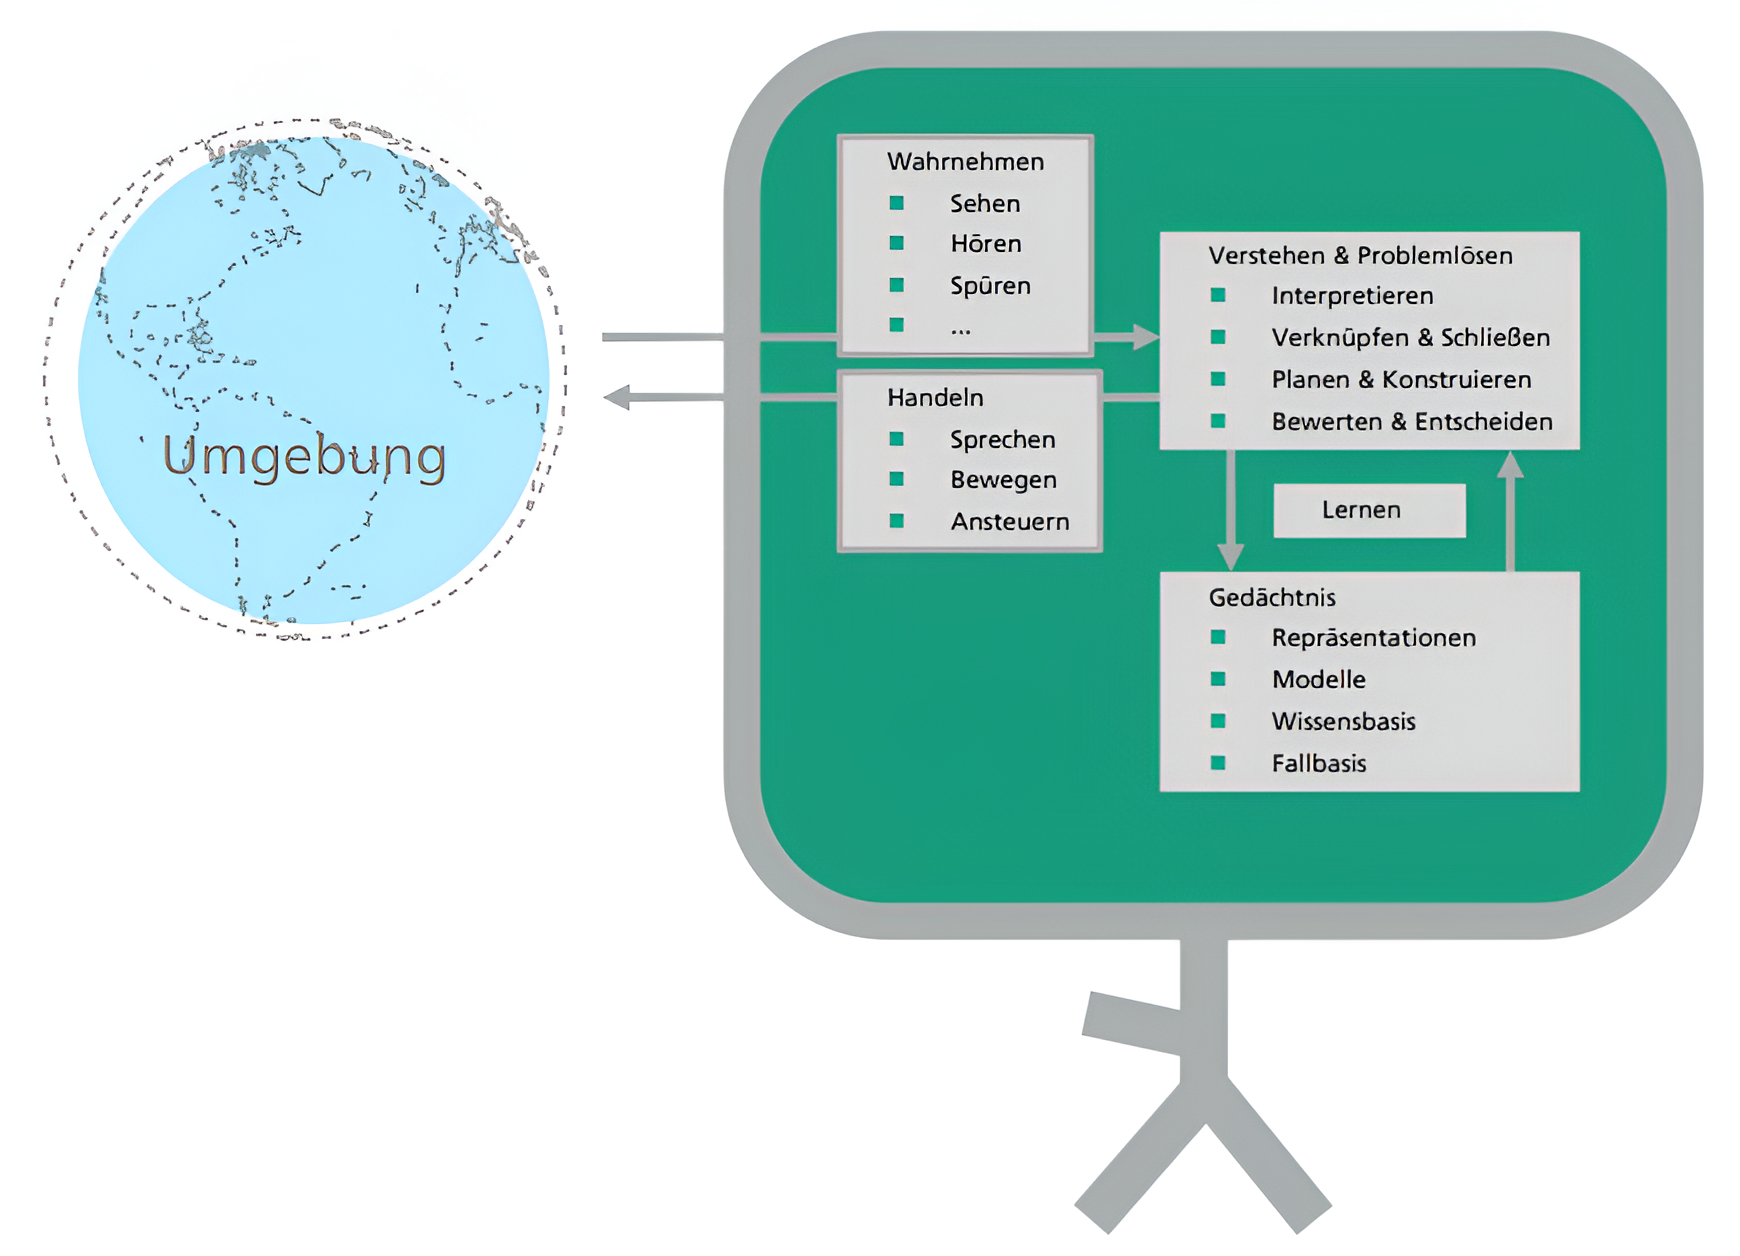
\includegraphics[width=0.75\linewidth]{./Bilder/Fraunhofer_KI-Umgebung.png}
    \caption{Interaktion eines KI-Systems mit seiner Umwelt (\cite{Hecker2018})}
    \label{fig:enter-label}
\end{figure}
\noindent Das Konzept hinter dieser KI besteht darin, dass Maschinen Fähigkeiten verwenden beziehungsweise imitieren können, die menschlich sind.\\
\\
Laut dem Fraunhofer Institut bilden sie kognitive Fähigkeiten ab.
Es scheint dabei, dass die Maschinen sich selbst und ihre Umgebung wahrnehmen und interpretieren können. Ihre Wahrnehmung und ihre Interpretation speist sich dabei auf Daten, Fakten, konkreten Modellen und Regeln, welche ihr nächstes Handeln bestimmen. Während des Nutzens lernen die Maschinen dabei kontinuierlich weiter. Sie besitzen ein Gedächtnis. Es gibt noch eine dritte Form der KI, die sogenannte Superintelligenz, diese wird es jedoch in nächster Zeit nicht geben.
%subsection allgemein (end)

\subsection{Bereiche der KI} % fold
\label{sec:bereicheDerKI}
Nachdem erklärt wurde um, was es sich bei KI handelt, ist es nun wichtig zu erklären, welche Bereiche und Teilgebiete es von KI gibt. Zu nennen sind dabei maschinelles Lernen, Neuronale Netze und Deep Learning (\cite{Bhatt2021}), (\cite{Hecker2018}), (\cite{Mocko2021}), (\cite{Roscher2025}) und (\cite{Zhu2021}).
Folgende Grafik zeigt anschaulich die einzelnen Teilgebiete der KI.
\begin{figure} [H]
    \centering
    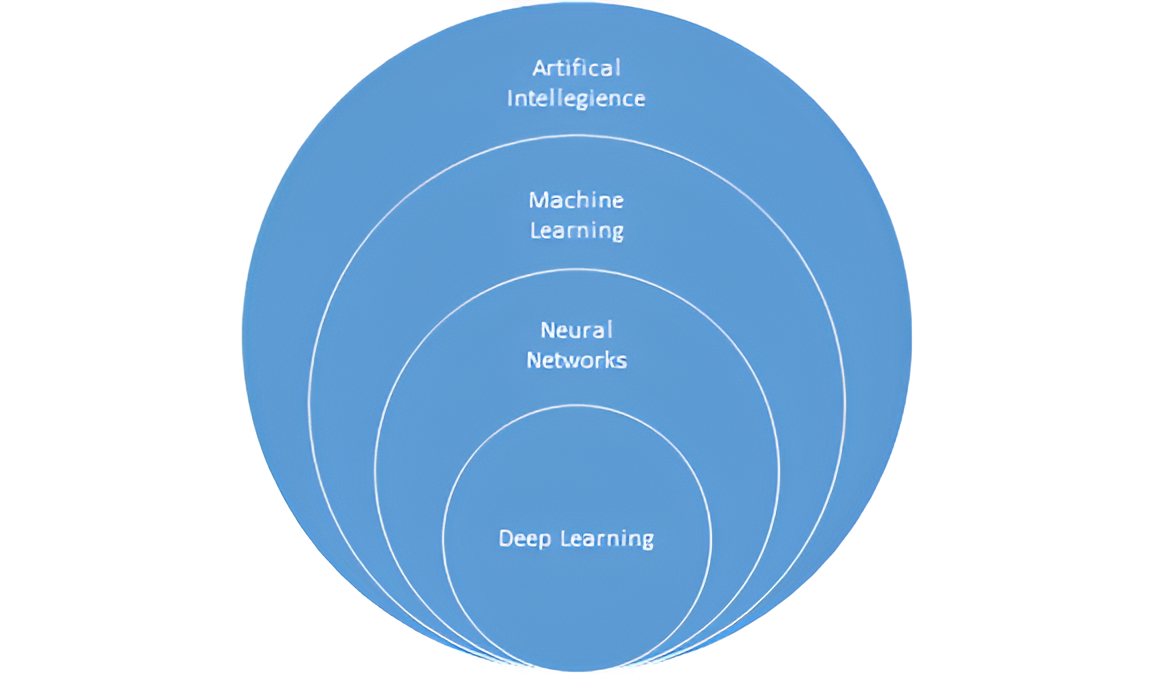
\includegraphics[width=0.75\linewidth]{./Bilder/Mocko_Die Beziehung zwischen KI, maschinellem Lernen, neuronalen Netzen und Deep Learning.png}
    \caption{Die Beziehung zwischen KI, maschinellem Lernen, neuronalen Netzen und Deep Learning (\cite{Mocko2021})}
    \label{fig:enter-label}
\end{figure}
\noindent KI beziehungsweise AI wird bereits in Kapitel 2.1.1 beschrieben und umfasst die anderen drei Bereiche. Die Grafik ist dabei so zu verstehen, dass der größere Kreis die jeweils kleineren Kreise umfasst, das heißt maschinelles Lernen ist ein Teil von KI, Neuronale Netze sind ein Teilgebiet von KI und von maschinellem Lernen und Deap Learning ist ein Teilgebiet von KI, von maschinellem Lernen und von Neuronalen Netzen. Im Folgenden werden nun die einzelnen Bereiche der KI erläutert.\\
\newpage
\noindent\textbf{\underline{Maschinelles Lernen:}}\\
\\
Maschinelles Lernen auf Englisch Machine Learning ist ein Teilgebiet der KI. Es beschreibt das Verfahren, in welchem Maschinen durch das Wiederholen von Aufgaben lernen. Dabei gibt es Algorithmen, welche mit Daten gefüttert werden und der Lernprozess ist eine Schleife, in welcher dieser wiederholt wird. Dadurch lernt die Maschine die Aufgabe zu lösen. Dies geschieht, in dem es Feedback erhält und so lernt, wie es die Aufgabe richtig löst. Es wird dabei kein Lösungsweg vorgegeben wie bei herkömmlichen Algorithmen, sondern die Maschine lernt durch Versuch und Irrtum beziehungsweise auf Englisch durch Trial and Error.\\
\\
\textbf{\underline{Neuronale Netze:}}\\
\\
Bei neuronalen Netzen handelt es sich um ein Teilgebiet des maschinellen Lernens. Idee der neuronalen Netze ist es, menschliche Neuronen nachzubilden und somit menschliches Denken nachzuahmen. Ein neuronales Netz besteht dabei aus Knoten die aneinander gereiht sind. Sie haben eine Eingabeschicht, ein Hidden Layer welches aus einer Neuronenschicht besteht und eine Ausgabeschicht die miteinander vernetzt sind. Sie trainieren ebenfalls in Schleifen und Durchgängen und werden durch das wiederholen besser und schneller.\\
\\
\textbf{\underline{Deep Learning:}}\\
\\
Deep Learing ist ein Teilgebiet der Neuronalen Netze. Sie sind dadurch gekennzeichnet, sie ein Hidden Layer besitzen, welches aus mehr als einer Neuronenschicht besteht (\cite{Bhatt2021}), (\cite{Dymatrix2018}) und (\cite{Zhu2021}). Folgende Grafik zeigt anschaulich ein Neuronales Netz und ein Deep Learning Netz.
\begin{figure} [H]
    \centering
    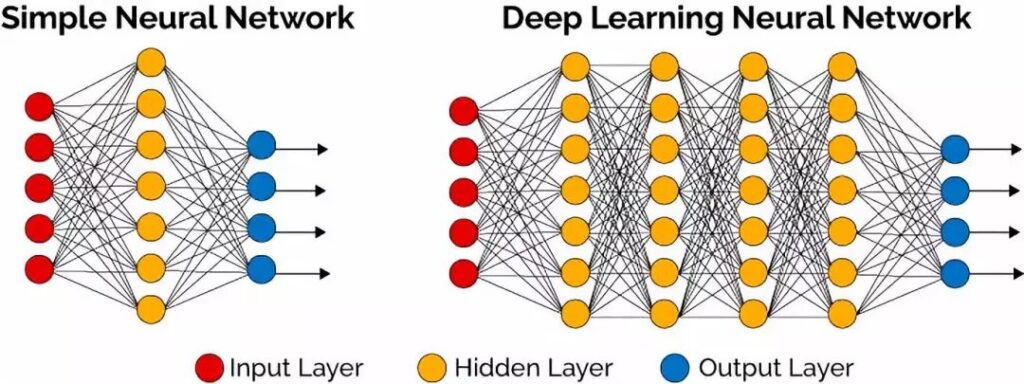
\includegraphics[width=0.75\linewidth]{./Bilder/Dymatrix_Deep_Learning_Networks.jpg}
    \caption{Deep Learning Network Grafik (\cite{Dymatrix2018})}
    \label{fig:enter-label}
\end{figure}
\noindent Sie können dabei Millionen Neuronenschichten beinhalten und dadurch immer komplexere Aufgaben lösen.\\
\\
Dies ist eine kurze Abhandlung über das Thema KI(\cite{Bhatt2021}), (\cite{Hecker2018}), (\cite{Mocko2021}), (\cite{Roscher2025}) und (\cite{Zhu2021}). Weitere wichtige KI-Bereiche wie LLM, Prompting und RAG werden in den Kapiteln 2.2 LLM, 2.3 Prompting und im Kapitel 2.4 erläutert, da diese eine wichtige Rolle in dieser Arbeit spielen.
%subsection bereicheDerKI (end)
% section KI (end)

\section{LLM} % (fold)
\label{sec:llm}
In dieser Arbeit wird/werden LLM(s) verwendet, über ihre Eigenschaften und Entwicklungen klärt dieses Kapitel auf

\subsection{Definition LLM} % fold
\label{sec:definitionLLM}
LLM ist ein Kombination aus zwei Bereichen der KI. Es ist ein Teilgebiet von Natural Language Processing (NLP), der Möglichkeit der Verarbeitung natürlicher Sprache, welche mit Hilfe der Trainingsmöglichkeit, welche Deep Learning bietet kombiniert. Folgende Grafik zeigt anschaulich, in welchem Gebiet LLM innerhalb der KI angesiedelt sind:

\begin{figure} [H]
    \centering
    \includegraphics[width=1\linewidth]{./Bilder/Hodiak_LLM und NLP Verschiedene Anwendungsfälle der Technologien.png}
    \caption{LLM und NLP Verschiedene Anwendungsfälle der Technologien (\cite{Hodiak2024})}
    \label{fig:enter-label}
\end{figure}
\noindent Dabei können diese Modelle durch das Training und der Verfügbarkeit von sehr großen Datenmengen, natürliche Sprache nachahmen. Ein bekanntes Beispiel für LLM sind Chatbots wie ChatGPT.
% section definitionLLM (end)

\subsection{Entwicklungen im Bereich LLM} % fold
\label{sec:entwicklungenImBereichLLM}
Im Bereich LLM gibt es schnelllebige Entwicklungen.\\
Viele LLM\\
Hugging Face\\
Eigene LLM entwickeln antrainieren\\
TODO QUELLEN finden ausschreiben
% section EntwicklungenImBereichLLM (end)

\section{Prompting} % (fold)
\label{sec:prompting}
Die Eingabe bzw. der Prompt ist ein wesentlicher Bestandteil, zum Nutzen von KI. Deshlalb ist es sehr wichtig diesen Begriff und die Vorgehensweisen, welche in dieser Arbeit getätigt werden zu erklären.

\subsection{Definition Prompting} % fold
\label{sec:definitionPrompting}
Unter dem Begriff Prompting versteht man folgendes:
TODO QUELLEN finden ausschreiben
% section definitionPrompting (end)

\subsection{Prompt Engineering und Prompt Techniken} % fold
\label{sec:promptEngineeringUndPromptTechniken}
Prompting ist wichtig im Umgang mit KI.\\
Prompt Engineering\\
Es gibt viele Prompt Techniken dabei bieten sich in dieser Arbeit folgende an um Testfälle zu generieren.
TODO QUELLEN finden ausschreiben
% section promptEngineeringUndPromptTechniken (end)
% section prompting (end)

\section{RAG} % (fold)
\label{sec:rag}
Bereits in Kapitel 1 Motivation wird RAG erwähnt. RAG ist für diese Arbeit von besonderer Wichtigkeit. 

\subsection{Definition RAG} % fold
\label{sec:definitionRAG}
RAG ist eine Technik, in welcher einem LLM Dokumente zur Verfügung gestellt werden. Dabei werden die in den Dokumenten enthaltenen Informationen für das LLM nutzbar gemacht (\cite{Gao2024}), (\cite{Honroth2024}), (\cite{Lewis2021}), (\cite{Miesle2023}), (\cite{Salemi2024}), (\cite{Schmid2024}) und (\cite{Wu2024}). Die Dokumente und Anfragen werden dabei in kleine Abschnitte, welche als Chunks bezeichnet werden, aufgeteilt. RAG lässt sich dabei in sehr vielen LLM anwenden und optimiert diese, ohne dass diese mit viel Aufwand trainiert werden müssen. Folgende Grafik zeigt anschaulich, wie RAG funktioniert:

\begin{figure} [H]
    \centering
    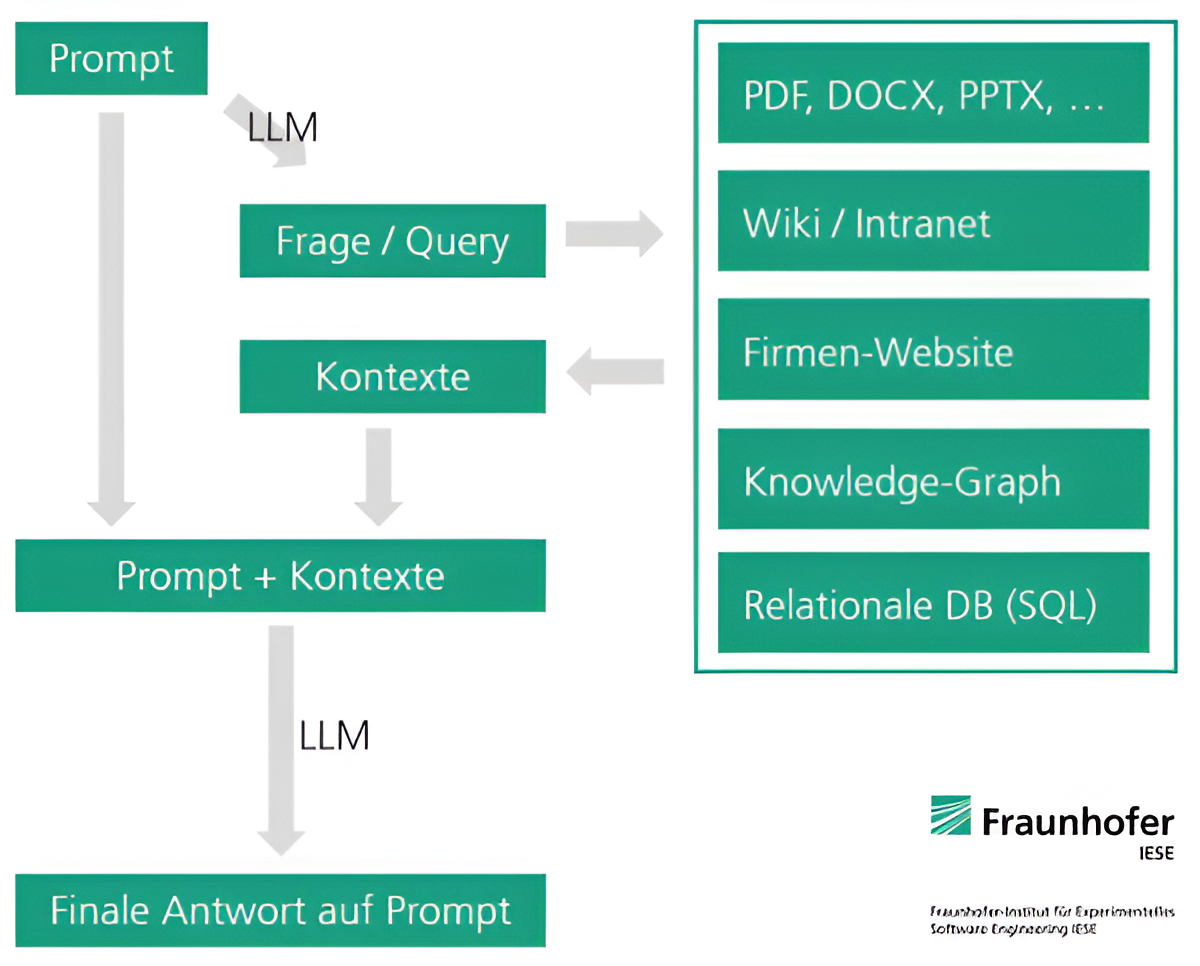
\includegraphics[width=0.75\linewidth]{./Bilder/Honroth_Wie funktioniert Retrieval Augmented Generation (RAG) im Detail.png}
    \caption{Wie funktioniert Retrieval Augmented Generation (RAG) im Detail (\cite{Honroth2024})}
    \label{fig:enter-label}
\end{figure}
\noindent Nun werden die einzelnen Schritte von RAG erklärt (\cite{Gao2024}), (\cite{Honroth2024}), (\cite{Lewis2021}), (\cite{Miesle2023}), (\cite{Salemi2024}), (\cite{Schmid2024}) und (\cite{Wu2024}):\\
\\
\textbf{\underline{Indexierung:}}\\
\\
Die Indexierung beschreibt den Prozess, wie die Daten aus einem Dokument in kürzere Abschnitte den Chunks aufgeteilt werden, um die Daten für die LLM verwertbar zu machen. Die Chunks werden maschinenlesbar gemacht und in einer Vektordatenbank gespeichert, aus welcher sie nun für die LLM zugreifbar sind. Sie werden vektorisiert.\\
\\
\textbf{\underline{Benutzereingabe:}}\\
\\
Die Benutzereingabe erfolgt als Prompt in natürlicher Sprache, welche sich auf die im Dokument befindlichen Daten beziehen.\\
\\
\textbf{\underline{Retrieval:}}\\
\\
Nachdem die Maschine die Eingabe erhalten hat und diese ebenfalls vektorisiert hat, wird mit der Methode des nächsten Nachbarn, wird die höchste Ähnlichkeit zwischen der Eingabe und der in der Vektordatenbank gespeicherten Chunks priorisiert.\\
\\
\textbf{\underline{Augmentation:}}\\
\\
Der LLM wird diese Kombination aus Prompt des Benutzers und der Kontext zu Verfügung gestellt.\\
\\
\textbf{\underline{Generation:}}\\
\\
Es wird nun eine Antwort generiert, welches die erhaltenen Informationen und das Training des jeweiligen LLM kombiniert.\\
\\
Wissenschaftliche Werke kommen zu dem Schluss, dass durch RAG LLM bessere Erlebnisse liefern können (\cite{Gao2024}), (\cite{Lewis2021}), (\cite{Salemi2024}) und (\cite{Wu2024}). Ergebnisse, welche RAG benutzen, zeichnen sich bei ihrer Performance aus und sind spezifischer und faktenreicher als Ergebnisse die nur von der LLM, ohne RAG erzeugt wurden.
% section definitionRAG (end)

\subsection{Einsatzmöglichkeiten von RAG} % fold
\label{sec:einsatzmöglichkeitenVonRAG}
RAG spielt in dieser Arbeit eine entscheidende Rolle. Mithilfe von RAG kann der LLM eine Anforderungsspezifikation zur Verfügung gestellt werden, aus welcher bereits manuell Anforderungstestfälle generiert wurden. Durch RAG kann die LLM diese Anforderungsspezifikation, welche eine PDF-Datei ist, gut verarbeiten und daraus Informationen ziehen. Dabei kann sie Informationen in Form von Text und von Bildern verarbeiten und berücksichtigen. Dies kann getrennt von einander geschehen, also PDF-Dateien sein, welche entweder nur Text oder Bilder enthalten, oder PDF-Dateien, welche Text und Bilder beinhalten.
% section einsatzmöglichkeitenVonRAG (end)
% section rag (end)

\section{Testfall} % (fold)
\label{sec:testfall}
In dieser Arbeit geht es um die Generierung von Testfällen durch KI. Es ist wichtig zu erklären was ein Testfall ist und welche Merkmale und Kriterien ein Testfall hat. 

\subsection{Definition Testfall} % fold
\label{sec:definitionTestfall}
Ein Testfall beschreibt folgendes.\\
Allgemein und auch Anforderungstestfall spezifisch
TODO QUELLEN finden ausschreiben
% section definitionTestfall (end)

\subsection{Aufbau eines Testfalls} % fold
\label{sec:aufbauEinesTestfalls}
Folgende Graphik zeigt ein Testfalldesign für eine SAP Applikation:

\begin{figure} [H]
    \centering
    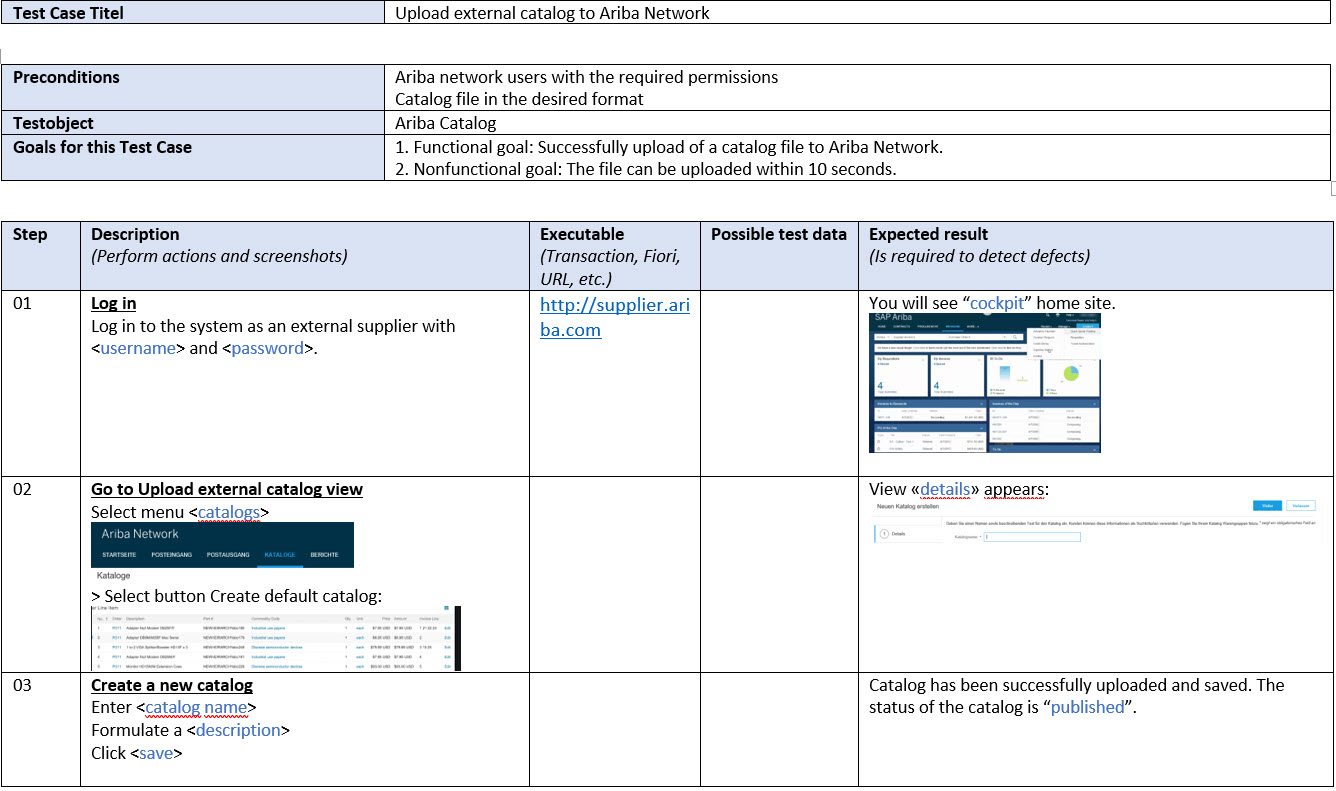
\includegraphics[width=1\linewidth]{./Bilder/Enderli_Testfall im SAP Solution Manager.jpg}
    \caption{Testfall im SAP Solution Manager (\cite{Enderli2019})}
    \label{fig:enter-label}
\end{figure}
\noindent Ein Testfall besitzt einen Namen, Vorbedingungen welche erfüllt sein müssen, damit der Testfall durchgeführt werden kann, Ziele die erreicht werden sollen. Der Testfall gliedert sich in Schritten, welche eine Beschreibung und ein erwartetes Ergebnis besitzen. In den Schritten wird somit überprüft, ob die Anwendung die Anforderungen erfüllt und somit das erwartete Ergebnis eintrifft. Testfälle können dabei positiv, als auch negativ sein. Bei negativen Testfällen wird überprüft ob das erwartete Ergebnis, wie erwartet nicht eintrifft, da die Voraussetzungen nicht erfüllt sind. In dieser Arbeit wird von der KI erwartet, dass es wenn es ein Testfall schreibt, diesen Aufbau einhält. Wenn sie es nicht macht, wird dies als negativ bewertet.
% section aufbauEinesTestfall (end)

\subsection{Testfallkriterien} % fold
\label{sec:testfallkriterien}
Folgende Werke zeigen Kriterien auf, welche Testfälle besitzen müssen.
% section testfallkriterien (end)
% section testfall (end)


\section{Anforderungsspezifikation} % (fold)
\label{sec:anforderungsspezifikation}
Eine Anforderungsspezifikation  ist das Fundament, aus welcher Testfälle erstellt werden. Ein Testfall überprüft ob die Anforderungen aus dieser Spezifikation erfüllt werden.

\subsection{Definition Anforderungsspezifikation} % fold
\label{sec:definitionAnforderungsspezifikation}
Eine Anforderungsspezifikation ist ein Dokument, welches alle Anforderungen beziehungsweise Requirements enthält, welche das System erfüllen muss und dessen Erfüllbarkeit und nicht Erfüllbarkeit mit Testfällen abgedeckt und getestet werden. Da sie der Grund für die Testfälle sind, müssen Anforderungsspezifikationen vollständig, präzise und in sich konsistent sein. Anforderungsspezifikationen enthalten System- und Benutzeranforderungen. Systemanforderungen beschreiben dabei die Benutzeranforderungen genau, wobei die Benutzeranforderungen funktionale und nicht funktionale Requirements besitzen. Folgende Grafik veranschaulicht anhand eines Beispiels, den Unterschied zwischen funktionalen und nicht funktionalen Requirements:

\begin{figure}[H]
    \centering
    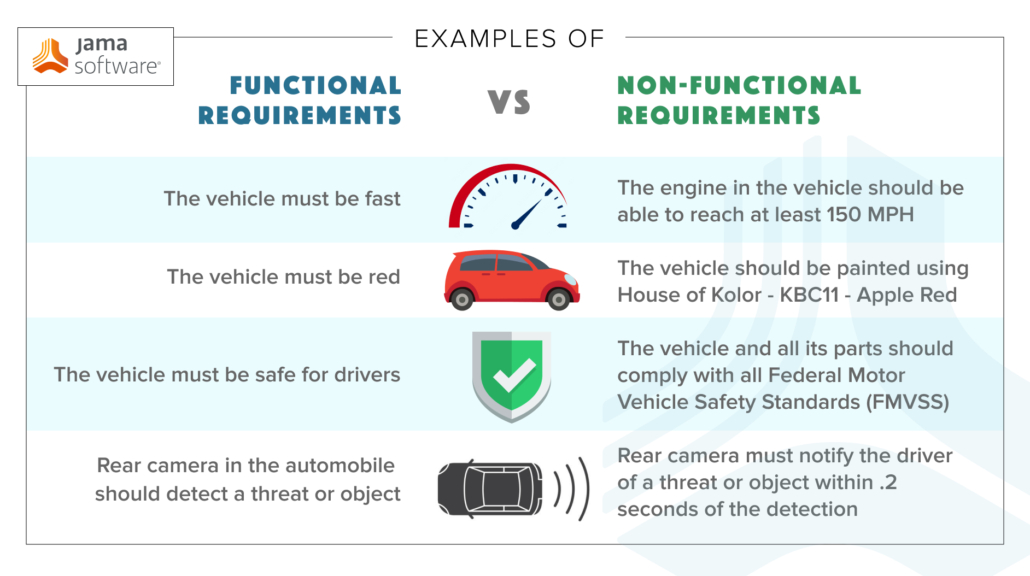
\includegraphics[width=0.75\linewidth]{./Bilder/Jama Software_Eigenschaften von funktionalen vs nichtfunktionalen Requirements.jpg}
    \caption{Eigenschaften von funktionalen vs nichtfunktionalen Requirements (\cite{JamaSoftware2024})}
    \label{fig:enter-label}
\end{figure}
\noindent Nicht funktionale Reuqirements beschreiben zum Beispiel Sicherheit, Wartung und Systemanforderungen. In dieser Arbeit geht es um funktionale Requirements, diese legen fest, was wie das System funktioniert und was passiert, wenn etwas im Positiven als auch wenn etwas im Negativen passiert. Den Unterschied erkennt man gut an der Grafik. Während die funktionellen Requirements festlegen, dass das Auto schnell sein und eine rote Farbe besitzen muss, legt die nicht funktionalen Requirements exakt fest, welche Geschwindigkeit das Auto erreichen und welchen genauen Rotton dieses besitzen muss. Funktionale Requirements dienen als Grundlage für die Testfallgenerierung durch die LLM in dieser Arbeit (\cite{Aysolmaz2018}), (\cite{Barmi2011}), (\cite{JamaSoftware2024}), (\cite{Mustafa2021}) und (\cite{Visure2024}).
% section definitionAnforderungsspezifikation (end)

\subsection{Bedeutung der Anforderungsspezifikation für die Testfallgenerierung} % fold
\label{sec:bedeutungDerAnforderungsspezifikationFürDieTestfallgenerierung}
In vielen Softwareprojekten werden Testfälle durch Requirements erzeugt (\cite{Aysolmaz2018}), (\cite{Barmi2011}), (\cite{JamaSoftware2024}), (\cite{Mustafa2021}) und (\cite{Visure2024}). Anforderungsspezifikationen dienen als Grundlage für die Testfallgenerierung durch die LLM in dieser Arbeit. Sie werden der LLM per RAG übermittelt und per Prompt dazu aufgerufen, Testfälle zu generieren, welche diese Requirements in Positiv- und Negativfällen abdecken. Dies ist essenziell für diese Arbeit, da es ohne Requirements nicht möglich ist, die von der LLM generierten Testfälle, auszuwerten. Mit ihrer Hilfe kann nun jedoch präzise festgestellt werden, wie diese im Bereich Vollständigkeit, Qualität und Fehlerhäufigkeit vorkommen.\\
\\
\textbf{\underline{Vollständigkeit:}}\\
\\
Werden alle Requirements, welche dem LLM übergeben werden, im positiven wie im negativen vollständig abgedeckt? Wenn Nein, wie viele werden ausgelassen?\\
\\
\textbf{\underline{Qualität:}}\\
\\
Werden alle Requirements präzise wiedergegeben und vollständig getestet, oder gibt es Rechtschreibfehler oder eine falsche Anordnung der Reihenfolge, oder werden Requirements aufgeteilt und falsch dargestellt?\\
\\
\textbf{\underline{Fehlerhäufigkeit:}}\\
\\
Wie viele Testschritte enthalten Informationen, welche sich nicht in der mitgegebenen Anforderungsspezifikation befinden und welche sind komplett frei erfunden und weisen keinen Zusammenhang mit dem System auf? So kann die Anzahl der Halluzinationen bestimmt und gezählt werden.
% section bedeutungDerAnforderungsspezifikationFürDieTestfallgenerierung (end)

\chapter{Related Work und aktuelle Forschung} % (fold)
\label{sec:relatedWorkUndAktuelleForschung}
Zum Thema KI im Allgemeinen und besonders im Hinblick auf Sprachmodelle zur Textgenerierung gibt es bereits viele wissenschaftliche Arbeiten (\cite{Iqbal2022}), (\cite{Yuan2021}), (\cite{Khan2024}), (\cite{Bhandari2024}), (\cite{Gu2024}), (\cite{Chen2024}) und (\cite{Wang2024}). Auf diese wird in diesem Kapitel näher eingegangen.\\
\\
Für den Einstieg zu dem Thema eignet sich ein wissenschaftliches Paper, welches einen Überblick bietet (\cite{Iqbal2022}). Dieses Paper stellt viele Deep Learning Modelle vor, die für die Generierung von Text verwendet wurden. Dabei werden die verschiedenen Modelle zusammengefasst und das Paper ermöglicht einen detaillierten Überblick über die Vergangenheit, Gegenwart und Zukunft von Textgenerierungsmodellen im Deep Learning. Die Autoren gehen davon aus, dass in Zukunft immer bessere Modelle entwickelt werden und dass die Forschung im Bereich der Texterzeugung weiter vorangetrieben wird. Das Paper macht jedoch auch deutlich, dass Modelle bei längeren Texten die natürliche Sprache noch nicht vollständig begriffen haben.\\
\\
Nicht nur die Textgenerierung durch KI ist wichtig, sondern auch die Auswertung des generierten Textes (\cite{Yuan2021}). Die Autoren stellten sich die Frage, wie man die generierten Texte nach Flüssigkeit, Genauigkeit und Effektivität beurteilen kann. Dafür entwickelten sie eine Metrik: Der sogenannte „BARTSCORE“ bewertet flexibel und unüberwacht aus unterschiedlichen Blickwinkeln. Unter anderem betrachtet er Informativität, Geläufigkeit oder Faktizität der generierten Texte. Die Autoren kommen zum Schluss, dass ihr Modell in 16 von 22 Settings besser abgeschnitten hat als andere gut bewertete Metriken.\\
\\
Ziel einer dieser Arbeiten ist es, einen Überblick über die Rolle von KI bei der Automatisierung von Softwaretests zu geben (\cite{Khan2024}). Die Autoren stellen die These auf, dass das Ziel der automatisierten Softwaretesterstellung mit KI möglich sein könnte. Im Werk werden zum Schluss entscheidende Schwierigkeiten, Probleme und Voraussetzungen vorgestellt. Am Ende bekräftigen die Autoren jedoch ihre These, dass das Testen von Software mit einer Reihe von Automatisierungsgadgets möglich sein könnte.\\
\\
Eine weitere Arbeit beschäftigt sich mit dem Potenzial der Anpassung von LLMs für den Bereich des Chip Testens (\cite{Bhandari2024}). Dabei sind funktionale Tests, die sich auf Testbenches stützen, wichtig für das Chipdesign. Es wird Feedback in die LLM eingegeben, um so die Testbench Generierung zu verbessern. Dies findet iterativ statt, um die Testabdeckung zu verbessern. Die Autoren nennen als Herausforderungen die Wiederholung der Antworten und die Feinabstimmung des LLM mit dem Umfang der Arbeit. Die Wertung der Testbenches in Bezug auf die Abdeckung gestaltet sich als nicht einfach. Trotzdem kommen sie zum Schluss, dass durch das Feedback die Testbenches besser verstanden werden. Ein entscheidender Faktor für die Qualität der Ausgabe ist dabei der Prompt.\\
\\
Weitere Werke beschäftigen sich mit dem Einsatz von KI bei der Erstellung von Unit Tests (\cite{Gu2024}). Die Autoren nennen drei mögliche Probleme bei der Erzeugung von Testfällen. 
Ein unzureichender Kontext, fehlende Test- und Abdeckungsinformationen und das Problem, dass LLM sich in Wiederholungsschleifen befinden können. Als Lösung bieten sie das Tool TestART an, welches eine Erfolgsquote von 78,55\% aufweist. In einer weiteren Arbeit wird ein Tool namens ChatUniTest vorgestellt, welches ebenfalls die Qualität von durch KI erzeugte Unit Tests verbessern soll (\cite{Chen2024}).\\
\\
Der aus Sprachmodellen generierte Code wirft Fragen im Bereich der Qualität und Korrektheit auf (\cite{Wang2024}). Die Autoren  gehen davon aus, dass sie Fehler im Code aufspüren können, indem sie Inkonsistenzen finden. Sie kommen zu dem Ergebnis, dass sie in der Lage sind, 75\% der von GPT-4 generierten fehlerhaften Programme zu erkennen, wobei sie eine Falsch Positiv Rate von 8,6\% haben. Die Autoren kommen zu der Erkenntnis, dass Entwickler möglicherweise nur eine sehr kleine Teilmenge des LLM generierten Codes untersuchen müssen, um die meisten Fehler zu finden. Die in der Arbeit vorgestellte Methodik dient als Inspiration, wie diese Arbeit aufgebaut ist.
% chapter relatedWorkUndAktuelleForschung (end)

\chapter{Methodik TODO Vorläufig muss überarbeitet werden!!!!} % (fold)
\label{sec:methodik}
Als Grundlage zur Erstellung von Testfällen dienen Anforderungsspezifikationen. Wichtig ist dabei, dass man sowohl Anforderungsspezifikationen als auch manuell erstellte Testfälle, die aus diesen Anforderungsspezifikationen erstellt wurden, findet.\\
\begin{figure} [h!]
    \centering
    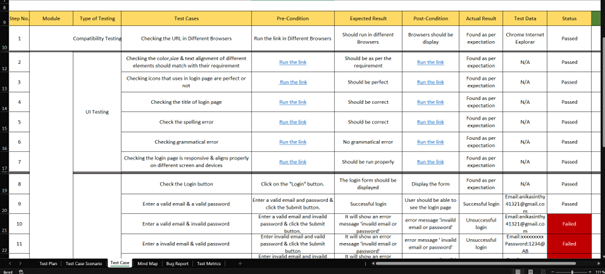
\includegraphics[width=1\linewidth]{./Bilder/Testspezifikationen.png}
    \caption{Eine Anforderungsspezifikation mit Informationen und Anweisungsschritten}
\end{figure}
\\
Nur so können diese Testfälle mit den KI generierten Testfällen valide verglichen und ausgewertet werden. Eine Quelle für Daten können Opensource Projekte auf Github sein, welche zu finden sind.\\
\newpage
\noindent Eine Anforderungsspezifikation enthält dabei Informationen und Anweisungsschritte, aus denen dann das LLM einen geeigneten Testfall generieren soll.\\
\begin{figure} [h!]
    \centering
    \includegraphics[width=1\linewidth]{./Bilder/Testfälle.png}
    \caption{Aus der Anforderungsspezifikation erzeugten manuelle Testfälle}
\end{figure}
\\
Nachdem die vorbereiteten Schritte abgeschlossen sind, beginnt der praktische Teil der Arbeit. Die Testfälle werden erzeugt und miteinander verglichen.\\
\\
Für die Auswertung der von der KI erstellten Testfällen und den Vergleich zwischen ihnen und den manuell erstellten Testfällen dient das Werk von (\cite{Wang2024}) als Inspiration. Für die Evaluation der erstellten Testfälle gibt es eine Metrik mit vier Kategorien:\\
\\
True Positives (TP)\\
False Positives (FP)\\
True Negatives (TN)\\ 
False Negatives (FN)\\
\\
In dieser Arbeit wird ChatGPT verwendet.\\
TODO AUSFORMULIEREN WARUM CHATGPT UND WELCHES MODELL WELCHE STATISTIKEN\\
\\
Wenn es LLM gibt, welche Testfälle generieren können, welche die Struktur und den Inhalt der Dokumente gut abdecken können, ist die Forschungsfrage positiv beantwortet. Am Ende werden die Ergebnisse kritisch eingeordnet und mögliche zukünftige Entwicklungen genannt.

\section{Verwendetes LLM} % (fold)
\label{sec:verwendetesLLM}
Dieser Abschnitt beschreibt das verwendete LLM, welche Eigenschaften es besitzt und aus welchen Gründen es für diese Arbeit verwendet wird.
TODO LLM beschreiben und Daten finden
% section verwendetesLLM (end)

\section{Testdaten} % (fold)
\label{sec:testdaten}
Die Testdaten welche für die Durchführung der Testfälle verwendet werden, werden in diesem Abschnitt erläutert.
TODO Testdaten beschreiben und zeigen
% section testdaten (end)

\section{Prompt und verwendete Methoden} % (fold)
\label{sec:promptUndVerwendeteMethoden}
Der Plan der vorliegenden Arbeit gestaltet sich wie folgt: Zuerst wird eine.
TODO Prompt zeigen und Methoden erklären
% section promptUndVerwendeteMethoden (end)

\section{Qualitätskriterien} % (fold)
\label{sec:qualitätskriterien}
Der Output der KI wird mit folgenden Qualitätskriterien bewertet:
TODO Qualitätskriterien finden, definieren und erläutern
% section qualitätskriterien (end)
% chapter methodik (end)

\chapter{Ergebnisse} % (fold)
\label{sec:ergebnisse}
In Kapitel 5 werden die Ergebnisse der von der KI erstellten Anforderungstestfälle dokumentiert, beschrieben und eingeordnet.

\section{Vorliegende Ergebnisse} % (fold)
\label{sec:vorliegendeErgebnisse}
Dies sind die Ergebnisse der KI
TODO Ergebnisse zeigen
% section vorliegendeErgebnisse (end)

\section{Auswertung der Ergebnisse} % (fold)
\label{sec:auswertungDerErgebnisse}
Die von der KI generierten Testfälle schneiden wie folgt ab:
TODO Ergebnisse auswerten und beschreiben
% section auswertungDerErgebnisse (end)

\section{Diskussion} % (fold)
\label{sec:diskussion}
Der Grund warum die Testfälle so abschneiden wie sie abschneiden, kann an folgenden Punkten liegen:
TODO Nach der Auswertung Ergebnisse einordnen und Grund dafür nennen
% section diskussion (end)
% chapter ergebnisse (end)

\chapter{Fazit und Ausblick} % (fold)
\label{sec:fazitUndAusblick}
Über die Einordnung der Ergebnisse dieser Arbeit und mögliche Bedeutungen für die Zukunft wird in Kapitel 6 Fazit und Ausblick Auskunft gegeben.
% chapter fazitUndAusblick (end)

\printbibliography
\newpage

\chapter*{Eidesstattliche Erklärung} % (fold)
\addcontentsline{toc}{chapter}{Eidesstattliche Erklärung}
\label{sec:eidesstattlicheErklärung}
Hiermit erkläre ich eidesstattlich, dass die vorliegende Arbeit von mir selbstständig und ohne unerlaubte Hilfe angefertigt wurde, insbesondere, dass ich alle Stellen, die wörtlich oder annähernd wörtlich oder dem Gedanken nach aus Veröffentlichungen und unveröffentlichten Unterlagen und Gesprächen entnommen worden sind, als solche an den entsprechenden Stellen innerhalb der Arbeit durch Zitate kenntlich gemacht habe, wobei in den Zitaten jeweils der Umfang der entnommenen Originalzitate kenntlich gemacht wurde. Ich bin mir bewusst, dass eine falsche Versicherung rechtliche Folgen haben wird.
\newline
\newline
\newline
\newline
\noindent
\begin{minipage}[t]{0.4\textwidth} 
    \centering 
    \rule{\textwidth}{0.4pt} \\ 
    Ort, Datum
\end{minipage}%
\hfill
\begin{minipage}[t]{0.4\textwidth} 
    \centering 
    \rule{\textwidth}{0.4pt} \\ 
    Unterschrift
\end{minipage}
% chapter eidesstattlicheErklärung (end)

\chapter*{Anhang} % (fold)
\addcontentsline{toc}{chapter}{Anhang}
\label{sec:anhang}
In diesem Anhang befinden sich die von der KI erzeugten Testfälle.

% chapter anhang (end)


\end{document}
